\subsection{Hồi quy tuyến tính đa biến}

Trước tiên ta kiểm tra sự phụ thuộc của biến delivery\_charges vào biến độc lập is\_expedited\_delivery. Ta sử dụng lệnh lm().

Kết quả phân tích trên Rstudio:
\begin{figure}[ht]
  \centering
  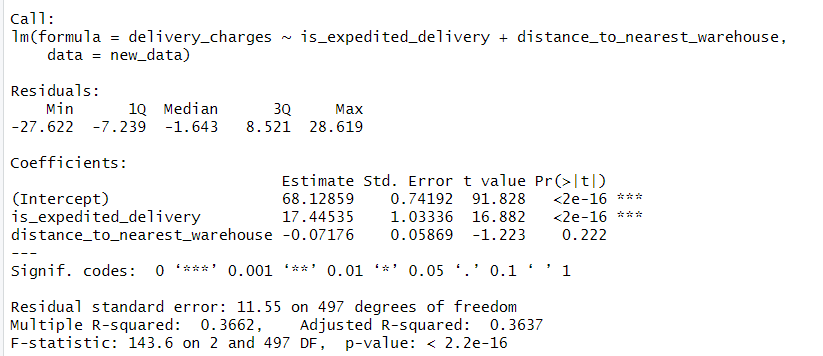
\includegraphics[width=0.7\linewidth]{graphics/5.5.1.png}
  \caption{Hồi quy tuyến tính model\_0 }
  \label{fig:your_label}
\end{figure}
\newpage
Với mức ý nghĩa 5\%, ta phân tích phần Coefficients (hệ số) như sau:

Định nghĩa biến x: is\_expedited\_delivery
, y:delivery\_charges

Cho biết hệ số của biến độc lập trong phương trình: $\beta_0= 67.9610, \beta_1= 17.4642 $
 Ta có phương trình hồi quy tuyến tính đơn giản: $y= 67.9610 + 17.4642x$

 Dựa vào bảng số liệu trên ta có:\\
 \begin{itemize}
 \item\textbf{Pr(>|t|)}: Các giá trị p-value đều nhỏ hơn 0.05, cho thấy cả hai hệ số đều có ý nghĩa thống kê trong mô hình.
\item\textbf{Multiple R-squared}: 0.3643, cho thấy mô hình giải thích được 36.43\% biến động của delivery\_charges.
 \end{itemize}

 Mô hình hồi quy này chỉ ra rằng việc giao hàng nhanh \textbf{(is\_expedited\_delivery)} có ảnh hưởng đáng kể và có ý nghĩa thống kê đến chi phí giao hàng \textbf{(delivery\_charges)}. Mặc dù mô hình giải thích được \textbf{36.43\%} biến động của chi phí giao hàng, điều này cho thấy vẫn còn nhiều yếu tố khác cần được xem xét để giải thích toàn bộ biến động của chi phí giao hàng.

Trên thực tế tổng giá trị đơn hàng phụ thuộc vào tổng giá trị mặt hàng, chi phí vận chuyển, mã giảm giá, khoảng cách đến kho hàng gần nhất.Vậy nên ta chọn biến \textbf{order\_total} làm biến phụ thuộc vào các biến độc lập \textbf{order\_price, delivery\_charges},\textbf{coupon\_discount} và \textbf{distance\_to\_nearest\_warehouse}.

Ta xét khi có các biến ngoại lai. Hồi quy tuyến tính mô hình trên ta có được:
\begin{figure}[ht]
  \centering
  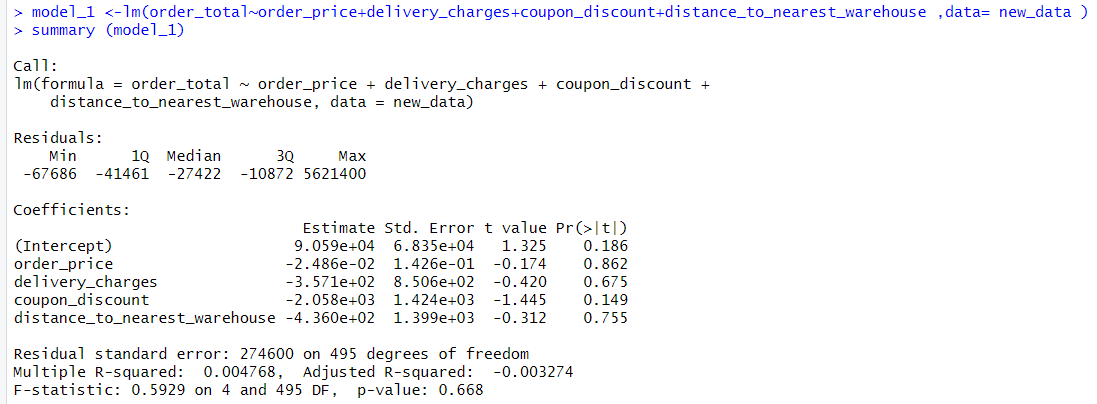
\includegraphics[width=0.7\linewidth]{graphics/5.5.2.png}
  \caption{Hồi quy tuyến tính model\_1 }
  \label{fig:your_label_1}
\end{figure}

Dựa trên kết qủa từ hàm \textbf{summary(model\_1)} ta rút ra nhận xét sau:
\begin{itemize}
\item \textbf{(Intercept)}: Khi tất cả các biến độc lập bằng 0, giá trị trung bình của order\_total là 90590. Tuy nhiên, giá trị p-value là 0.186, không có ý nghĩa thống kê.
\item \textbf{order\_price}: Hệ số ước lượng là -0.02486, và p-value là 0.862, không có ý nghĩa thống kê.
\item \textbf{delivery\_charges}: Hệ số ước lượng là -357.1, và p-value là 0.675, không có ý nghĩa thống kê.
\item \textbf{coupon\_discount}: Hệ số ước lượng là -2058.0, và p-value là 0.149, không có ý nghĩa thống kê.
\item \textbf{distance\_to\_nearest\_warehouse}: Hệ số ước lượng là -436.0, và p-value là 0.755, không có ý nghĩa thống kê.
\item\textbf{Multiple R-squared}: 0.004768, chỉ ra rằng mô hình chỉ giải thích được 0.4768\% biến động của order\_total.
\item\textbf{F-statistic}: 0.5929, với p-value là 0.668, cho thấy mô hình tổng thể không có ý nghĩa thống kê
\end{itemize}
Mô hình hồi quy model\_1 không phù hợp tốt với dữ liệu của bạn bởi vì:
\begin{itemize}
\item Các biến độc lập đều không có ý nghĩa thống kê ($p-value > 0.05$).
\item Chỉ số \textbf{R-squared} rất thấp, cho thấy mô hình không giải thích được biến động của order\_total.
\item\textbf{F-statistic} không có ý nghĩa thống kê, gợi ý rằng mô hình tổng thể không phù hợp.
\end{itemize}

Tiếp theo ta xét tiếp khi bỏ các giá trị ngoại lai

Hồi quy trên Rstudio ta có được:
\begin{figure}[ht]
  \centering
  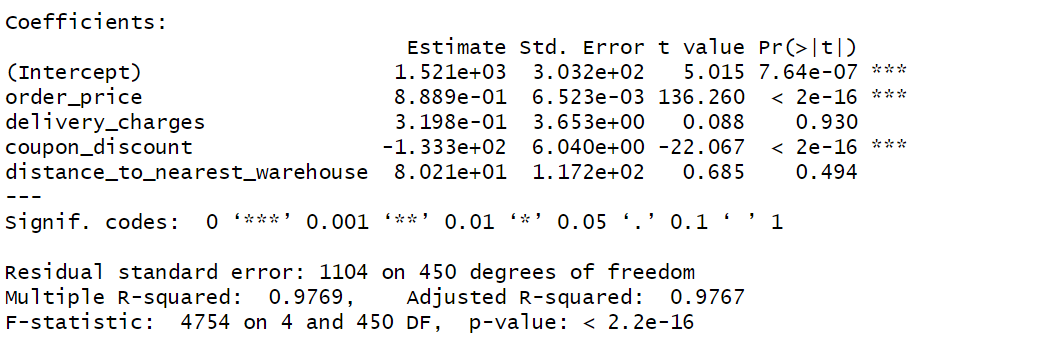
\includegraphics[width=0.7\linewidth]{graphics/5.5.3.png}
  \caption{Hồi quy tuyến tính model\_2 }
  \label{fig:your_label_2}
\end{figure}

Dựa trên kết quả từ hàm \textbf{summary(model\_2)}, ta có thể rút ra các nhận xét:

Với mức ý nghĩa 5\%, ta phân tích phần Coeficients(hệ số) như sau:

Định nghĩa các biến:  y: order\_total, $x_1$: order\_price, $x_2$: delivery\_charges, $x_3$: coupon\_discount, $x_4$: distance\_to\_nearest\_warehouse.

Cho các hệ số của từng biến độc lập trong phương trình : $\beta_0= 1450, \beta_1= 0.8887, \\\beta_2= 1.132, \beta_3= -133.9, \beta_4= 103.1$ Ta có phương trình hồi quy: 

 \hspace{25mm}$y= 1450 + 0.8887x_1 + 1.132x_2 - 133.9x_3 + 103.1x_4$

Ý nghĩa của hệ số hồi quy:
\begin{itemize}
\item\textbf{(Intercept)}: Khi tất cả các biến độc lập bằng 0, giá trị trung bình của order\_total là 1450.0. Giá trị p-value rất nhỏ (1.57e-05), có ý nghĩa thống kê.
\item\textbf{order\_price}: Hệ số ước lượng là 0.8887, và p-value rất nhỏ (< 2e-16), có ý nghĩa thống kê mạnh mẽ. Mỗi đơn vị tăng của order\_price dẫn đến order\_total tăng trung bình 0.8887 đơn vị, giữ nguyên các yếu tố khác.\\
\item\textbf{delivery\_charges}: Hệ số ước lượng là 1.132, và p-value là 0.776, không có ý nghĩa thống kê.
\item\textbf{coupon\_discount}: Hệ số ước lượng là -133.9, và p-value rất nhỏ (< 2e-16), có ý nghĩa thống kê mạnh mẽ. Mỗi đơn vị tăng của coupon\_discount dẫn đến order\_total giảm trung bình 133.9 đơn vị, giữ nguyên các yếu tố khác.
\item\textbf{distance\_to\_nearest\_warehouse}: Hệ số ước lượng là 103.1, và p-value là 0.399, không có ý nghĩa thống kê.
\end{itemize}

Chỉ số đo lường của mô hình:

\begin{itemize}
\item\textbf{Multiple R-squared}: 0.9765, cho thấy mô hình giải thích được 97.65\% biến động của order\_total.
\item\textbf{F-statistic}: 4534, với p-value < 2.2e-16, cho thấy mô hình tổng thể có ý nghĩa thống kê mạnh mẽ.
\end{itemize}

Từ 2 mô hình trên ta có thể thấy được rằng giá trị ngoại lai ảnh hưởng đến hồi quy tuyến tính như thế nào. Các giá trị ngoại lai có thể làm suy yếu mô hình hồi quy tuyến tính, làm giảm khả năng giải thích của mô hình và làm sai lệch các hệ số ước lượng. Sau khi xử lý ngoại lai, mô hình có sự cải thiện rõ rệt, với giá trị R-squared cao hơn và các biến có ý nghĩa thống kê tốt hơn. Việc loại bỏ các ngoại lai giúp làm sạch dữ liệu và cải thiện độ chính xác của mô hình.

Qua mô hình 2 ta thấy có hai biến là biến \textbf{order\_price} và \textbf{coupon\_discout} là phù hợp (p-value<0.05), vì thế nên ta loại bỏ hai biến còn lại ra khỏi mô hình.

Loại bỏ hai biến \textbf{delivery\_charges} và \textbf{distance\_to\_nearest\_warehouse}, giữ lại biến có ý nghĩa là \textbf{order\_price} và \textbf{coupon\_discount}.

Từ đó ta có mô hình 3 : $y= \beta_0 + \beta_1x_1 + \beta_2x_2$ với y: order\_total, $x_1$: order\_price, $x_2$: coupon\_discount.

Ta tiếp sử dụng Rstudio để phân tích mô hình 3
\begin{figure}[ht]
  \centering
  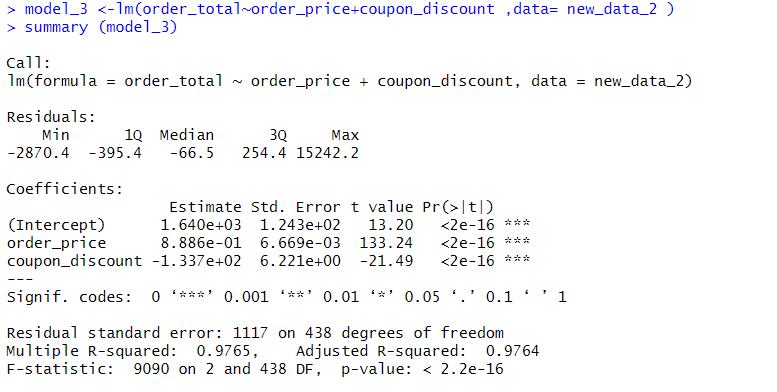
\includegraphics[width=0.7\linewidth]{graphics/5.5.4.png}
  \caption{Hồi quy tuyến tính model\_3 }
  \label{fig:your_label_1}
\end{figure}

Với mức ý nghĩa 5\% ta có phương trình: $y= 1640 + 0.8886x_1 - 133.7 x_2$

Ý nghĩa của hệ số hồi quy:
\begin{itemize}
\item\textbf{(Intercept)}: Hệ số chặn (Intercept) là 1640, có ý nghĩa thống kê mạnh (p-value < 0.001).
\item\textbf{order\_price}: Hệ số của order\_price là 0.8886, có ý nghĩa thống kê mạnh với p-value rất nhỏ (< 0.001). Điều này cho thấy mối quan hệ tích cực giữa order\_price và order\_total, tức là khi giá trị đơn hàng tăng, tổng giá trị đơn hàng cũng tăng.
\item\textbf{coupon\_discount}: Hệ số của coupon\_discount là -133.7, có ý nghĩa thống kê mạnh với p-value < 0.001. Mối quan hệ này cho thấy khi mức giảm giá (coupon) tăng lên, tổng giá trị đơn hàng giảm đi.
\end{itemize}

Chỉ số đo lường mô hình:

\begin{itemize}
\item\textbf{Multiple R-squared}: 0.9765, cho thấy mô hình giải thích được 97.65\% biến động của order\_total.
\item\textbf{F-statistic}: 9090, với p-value < 2.2e-16, cho thấy mô hình tổng thể có ý nghĩa thống kê mạnh mẽ.
\end{itemize}

Mô hình 3 có hiệu quả rất cao trong việc giải thích sự biến thiên của \textbf{order\_total}, với \textbf{R-squared} lên đến \textbf{97.65\%}. Các biến \textbf{order\_price} và \textbf{coupon\_discount} là những yếu tố quan trọng và có ảnh hưởng rõ rệt đến tổng giá trị đơn hàng. Việc loại bỏ các biến không quan trọng như \textbf{delivery\_charges} và \textbf{distance\_to\_nearest\_warehouse} giúp đơn giản hóa mô hình mà vẫn giữ được khả năng dự đoán chính xác.

Tiếp tục kiểm định, ta xác định khoảng tin cậy cho hệ số với mức ý nghĩa 5\%\ bằng lệnh \textbf{confint(model\_3)}:
\begin{figure}[ht]
  \centering
  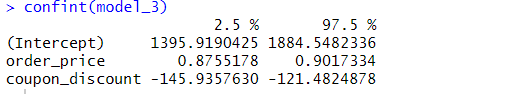
\includegraphics[width=0.7\linewidth]{graphics/5.5.5.png}
  \caption{Kiểm định khoảng tin cậy hệ số model\_3 }
  \label{fig:your_label_1}
\end{figure}

Ta thấy các hệ số $\beta_0= 1640\in(1395.91904; 1884.5482), \beta_1= 0.8886\in(.8755;0.9017),\\ \beta_2= -133.7\in(-145.9358 -121.4825)$

Kiểm tra giả định mô hình hồi quy tuyến tính bằng đồ thị:

\begin{figure}[h]
  \centering
  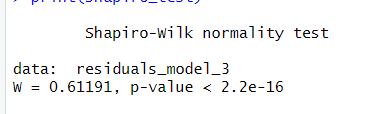
\includegraphics[width=0.5\linewidth]{graphics/5.5.6.png}
  \caption{Đồ thị kiểm định mô hình hồi quy  tuyến tính }
  \label{fig:your_label_1}
\end{figure}
\newpage
Nhận xét dựa trên đồ thị chuẩn đoán:\\
\textbf{Residual vs Fitted:}
\begin{itemize}
 \item Các điểm dữ liệu không hoàn toàn phân bố ngẫu nhiên quanh đường ngang tại 0, gợi ý rằng có thể có vấn đề với tuyến tính hoặc phương sai không đồng nhất. 
\end{itemize}
 \textbf{Q-Q Residuals:}
 \begin{itemize}
\item Các điểm dữ liệu phần lớn nằm dọc theo đường chéo, nhưng có một số điểm lệch ở hai đầu Điều này gợi ý rằng phần dư có thể không hoàn toàn tuân theo phối chuẩn, nhưng sự sai lệch không quá nghiêm trọng.
 \end{itemize}
\textbf{Scale-Location:}
\begin{itemize}
\item Các điểm dữ liệu không hoàn toàn phân bố ngẫu nhiên và có xu hướng tăng lên, điều này gợi ý rằng phương sai có thể không đồng nhất.
\end{itemize}
\textbf{Residuals và Leverage:}
\begin{itemize}
\item Một số điểm có leverage cao và phần dư lớn, cho thấy một số điểm dữ liệu  có thể có ảnh hưởng mạnh đến mô hình. Những điểm này cần được kiểm tra kỹ lưỡng.
\end{itemize}
\textbf{Kết luận:}

Mô hình 3 có độ phù hợp tương đối tốt với dữ liệu, với \textbf{R-squared} cao và các biến độc lập có ý nghĩa thống kê.

Đồ thị chẩn đoán cho thấy một số vấn đề tiềm ẩn về tuyến tính, phương sai đồng nhất và phân phối chuẩn của phần dư. Mặc dù có một số điểm cần lưu ý, nhưng chúng không quá nghiêm trọng.

Có thể kết luận rằng mô hình 3 tương đối đúng và phù hợp để dự đoán \textbf{order\_total}. Tuy nhiên, cần kiểm tra thêm và có thể thực hiện một số điều chỉnh nhỏ để cải thiện thêm độ chính xác của mô hình.







